\section{Methods}
\label{sec:methods}
In this section we will descripe the different theories and techniques outlined in Section \ref{sec:background}, in deeper algorithmic detail. 

\subsection{Goal Ordering / Prioritisation}
\label{methods:goal_ordering}
As mention in section \ref{sec:background}, the technique we use for prioritising/ordering which goal to fulfill first, is of our own design. In oder to explain how the algorithm functions, we will break it down into three seperate steps. For the \textbf{first} step, lets consider an example set of goal cells, which are all only accessible form a single entrance. 
\break
% Example of cells 
\begin{figure}[ht!]
\centering
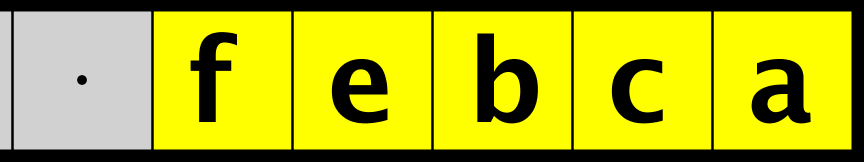
\includegraphics[width=50mm]{graphics/ie_level.png}
\caption{Goal set with single entrance\label{fig:sample}}
\end{figure}

For the example in Figure \ref{fig:sample}, the optimal ordering would be to fulfill the goals in the following order: \textbf{a, c, b, e, f} from first to last. To accomplish this, our algorithm provides an ordering score to each goal. First it searches through each goal, evaluating its 8 neighboring cells, including the diagonal neighbors. For every neighbor cell that is also a goal, the score of the cell is incremented by 1. For every free neighbor cell, it is incremented by a score of 2. In Figure \ref{fig:grid1}, the checking of neighbor cells is illustrated with a grid. The middle cell is the one currently being checked, while the green represents a neighbor goal. The red cell represent either walls or space outside the level. 

% Example of scoring 
\begin{figure}[ht!]
\centering
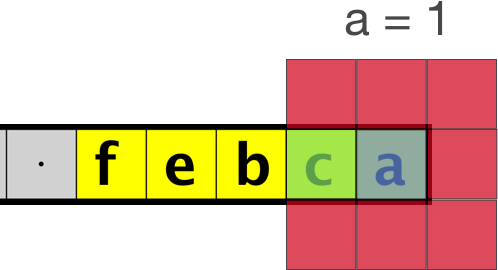
\includegraphics[width=50mm]{graphics/goal_pri_1.png}
\caption{Neighbor checking of goal a\label{fig:grid1}}
\end{figure}

The goal \textbf{a} is given a start score of 1. Goal \textbf{f} and \textbf{b} are given scores of respectively 3 and 2 as can be seen in Figure \ref{fig:grid2}. The blue cell in the grid represents a free cell and therefore a score increment of 2. The remaining goals not shown in the figures are all given a score of 2. 

% Example of scoring 
\begin{figure}[ht!]
\centering
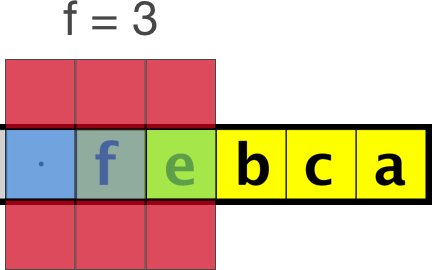
\includegraphics[width=50mm]{graphics/goal_pri_3.png}
\break
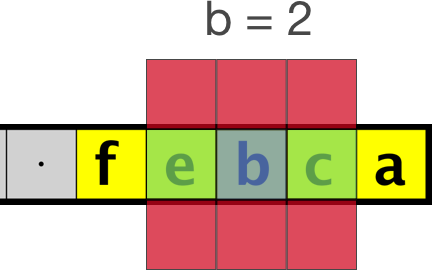
\includegraphics[width=50mm]{graphics/goal_pri_2.png}
\caption{Neighbor checking of goal f and b\label{fig:grid2}}
\end{figure}

After scoring the goals according to their neighbors, we reach the \textbf{second} step of the ordering algorithm. In this step we create a matrix, with the height and width equal to the number of goals. Each column of the matrix will represent a goal cell and the first row will the ordering scores from previously. 

\begin{table}[!htb]
	\label{tab:example_matrix}
    \caption{\centering Example level - Ordering matrix \break Incomplete(left) \& Complete (right)}
	\begin{minipage}{.5\linewidth}
      \centering
	  	\label{fig:scores_2}
		\begin{tabular}{lllll}
		\hline
		\textbf{f} & \textbf{e} & \textbf{b} & \textbf{c} & \textbf{a} \\ \hline
		3          & 2          & 2          & 2          & 1          \\ 
		-          & -          & -          & -          & -          \\ 
		-          & -          & -          & -          & -          \\ 
		-          & -          & -          & -          & -          \\ 
		-          & -          & -          & -          & -          \\ \hline
		\end{tabular}
    \end{minipage}%
    \begin{minipage}{.5\linewidth}
      \centering
		\label{fig:scores_2}
		\begin{tabular}{lllll}
		\hline
		\textbf{f} & \textbf{e} & \textbf{b} & \textbf{c} & \textbf{a} \\ \hline
		3          & 2          & 2          & 2          & 1          \\ 
		4          & 2          & 3          & 2          & 1          \\ 
		5          & 3          & 3          & 2          & 1          \\ 
		6          & 4          & 3          & 2          & 1          \\ \hline
		\textbf{7} & \textbf{4} & \textbf{3} & \textbf{2} & \textbf{1} \\ \hline
		\end{tabular}
    \end{minipage} 
\end{table}


When the matrix has been created as seen in Figure \ref{tab:example_matrix} (left), the algorithm increments the scores such that no scores are the same after all iterations. This is done by comparing the previous scores to each other. It increments from the direction of the heighest beginning score, which can cause issues is some level structures, but has been found to work for most cases. The last row of the matrix will then contain the final ordering scores of the goals. In cases where different groups of exist in the same level, the algorithm will allow for some scores to be the same, such that the different groups of goals can be ordered independently, without one having to be filled before the other. 

The last row of the matrix in Figure \ref{tab:example_matrix} (right), is now used to order the goals. The goals with the least ordering score will be prioritised first, because they are assumed to be non-blocking of others. The \textbf{third} and last step of the algoritm is the acutal sorting of the goals based on the ordering scores. For every time a box has been placed on a goal, this algorithm is repeated to take new boxes and agents into account. 

\emph{How does your client work? Describe its overall algorithmic functionality as clearly and precisely as possible, without going into any implementation details.  Describe it in terms of the theories you rely on (as presented in background). Include small, illustrative examples of how the client works. Aim to describe your client suffi- ciently precisely that a reader being an expert in the field would be able to implement a similar solution based on your description (note that this is not an encouragement to describe implementation details, but rather make sure that the overall structure and ideas of your implementation are sufficiently precise).}
